%%% License: Creative Commons Attribution Share Alike 4.0 (see https://creativecommons.org/licenses/by-sa/4.0/)


%%%%%%%%%%%%%%%%%%%%%%%%%%%%%%%%%%%%%%%%%

%----------------------------------------------------------------------------------------
%	PACKAGES AND OTHER DOCUMENT CONFIGURATIONS
%----------------------------------------------------------------------------------------

\documentclass{article}

\usepackage{amssymb}
\usepackage{enumerate}
\usepackage[usenames,dvipsnames]{color}
\usepackage{fancyhdr} % Required for custom headers
\usepackage{lastpage} % Required to determine the last page for the footer
\usepackage{extramarks} % Required for headers and footers
\usepackage[usenames,dvipsnames]{color} % Required for custom colors
\usepackage{graphicx} % Required to insert images
\usepackage{listings} % Required for insertion of code
\usepackage{courier} % Required for the courier font
\usepackage[table]{xcolor}
\usepackage{amsfonts,amsmath,amsthm,parskip,setspace,url}
\usepackage[section]{placeins}
\usepackage[a4paper]{geometry}
\usepackage[USenglish]{babel}
\usepackage[utf8]{inputenc}
\usepackage{hyperref}
\usepackage{subfig}


% Margins
\topmargin=-0.45in
\evensidemargin=0in
\oddsidemargin=0in
\textwidth=6.5in
\textheight=9.0in
\headsep=0.6in

\linespread{1.1} % Line spacing

%----------------------------------------------------------------------------------------
%	DOCUMENT STRUCTURE COMMANDS
%	Skip this unless you know what you're doing
%----------------------------------------------------------------------------------------

% Header and footer for when a page split occurs within a problem environment
\newcommand{\enterProblemHeader}[1]{
\nobreak\extramarks{#1}{#1 continued on next page\ldots}\nobreak
\nobreak\extramarks{#1 (continued)}{#1 continued on next page\ldots}\nobreak
}

% Header and footer for when a page split occurs between problem environments
\newcommand{\exitProblemHeader}[1]{
\nobreak\extramarks{#1 (continued)}{#1 continued on next page\ldots}\nobreak
\nobreak\extramarks{#1}{}\nobreak
}

\setcounter{secnumdepth}{0} % Removes default section numbers
\newcounter{homeworkProblemCounter} % Creates a counter to keep track of the number of problems

\newcommand{\homeworkProblemName}{}
\newenvironment{ex}[1][Problem \arabic{homeworkProblemCounter}]{ % Makes a new environment called homeworkProblem which takes 1 argument (custom name) but the default is "Problem #"
\stepcounter{homeworkProblemCounter} % Increase counter for number of problems
\renewcommand{\homeworkProblemName}{#1} % Assign \homeworkProblemName the name of the problem
\section{\homeworkProblemName} % Make a section in the document with the custom problem count
\enterProblemHeader{\homeworkProblemName} % Header and footer within the environment
}{
\exitProblemHeader{\homeworkProblemName} % Header and footer after the environment
}

\newcommand{\problemAnswer}[1]{ % Defines the problem answer command with the content as the only argument
\noindent\framebox[\columnwidth][c]{\begin{minipage}{0.98\columnwidth}#1\end{minipage}} % Makes the box around the problem answer and puts the content inside
}

\newcommand{\homeworkSectionName}{}
\newenvironment{homeworkSection}[1]{ % New environment for sections within homework problems, takes 1 argument - the name of the section
\renewcommand{\homeworkSectionName}{#1} % Assign \homeworkSectionName to the name of the section from the environment argument
\subsection{\homeworkSectionName} % Make a subsection with the custom name of the subsection
\enterProblemHeader{\homeworkProblemName\ [\homeworkSectionName]} % Header and footer within the environment
}{
\enterProblemHeader{\homeworkProblemName} % Header and footer after the environment
}

\newif\ifsolutions

%----------------------------------------------------------------------------------------
%----------------------------------------------------------------------------------------
%----------------------------------------------------------------------------------------
% Set up the header and footer
\pagestyle{fancy}
\lhead[c]{\textbf{{\color[rgb]{.5,0,0} K{\o}benhavns\\Universitet }}\\} % Top left header
\chead{\textbf{{\color[rgb]{.5,0,0} \Class }}\\ \hmwkTitle \\ \firstxmark} % Top center head
\rhead{\instructor \\ \theprofessor \\} % Top right header
\lfoot{\lastxmark} % Bottom left footer
\cfoot{} % Bottom center footer
\rfoot{Page\ \thepage\ of\ \protect\pageref{LastPage}} % Bottom right footer
\renewcommand\headrulewidth{0.4pt} % Size of the header rule
\renewcommand\footrulewidth{0.4pt} % Size of the footer rule

\setlength\parindent{12pt} % Removes all indentation from paragraphs







%----------------------------------------------------------------------------------------
%	NAME AND CLASS SECTION
%----------------------------------------------------------------------------------------

\newcommand{\hmwkTitle}{Note on Battaglini (2003)} % Assignment title
\newcommand{\Class}{Mechanism Design} % Course/class
\newcommand{\instructor}{Fall 2020} % TA
\newcommand{\theprofessor}{Prof. Egor Starkov} % Professor

%\theoremstyle{definition} \newtheorem{ex}{\textbf{\Large{Exercise & #}\\}}
\setlength{\parskip}{5 pt}




















\begin{document}

\begin{center}
	{\Huge Extracting Correlated Information Without Transfers}
\end{center}
\bigskip

This note explains how equilibrium works in the model of Battaglini (2003) and how to find it. For model setup, see M4 slide deck.

The equilibrium is described by a profile of strategies for all players, $(a,m_1,m_2)$, where $a(m_1,m_2)$ is the principal's choice of action given messages, and $m_i(\omega)$ is the agent $i$'s choice of message given the true state. The principal chooses $a$ to maximize his expected payoff $\mathbb{E}_\omega [u_p(a,\omega)|m_1,m_2]$ conditional on the two reports $(m_1,m_2)$, where $u_p(a,\omega) = -\left(\left\| a - \omega \right\|_2\right)^2$. Therefore, his equilibrium strategy must be given by
\begin{align}
	a^*(m_1,m_2) \equiv \mathbb{E} \left[ \omega | m_1, m_2 \right]
	\label{eq:optact}
\end{align}

In other words, by changing their reports $m_i$, the agents can directly affect the principal's choice of action. Our mission of finding a fully revealing equilibrium thus lies in designing communication strategies $m_i(\omega)$ in such a way that:
\begin{enumerate}
	\item $a^*(m_1(\omega),m_2(\omega)) = \omega$, i.e. the two messages allow to identify the state;
	\item $m_i(\omega) \in \arg \max_{\hat{m}_i} \left\{ -\left(\left\| a^*(\hat{m}_i,m_j(\omega)) - (\omega + b_i) \right\|_2\right)^2 \right\}$, i.e. $m_i(\omega)$ should be optimal for agent $i$.
\end{enumerate}

\begin{figure}[b!]
	\centering
	\parbox{7cm}{
		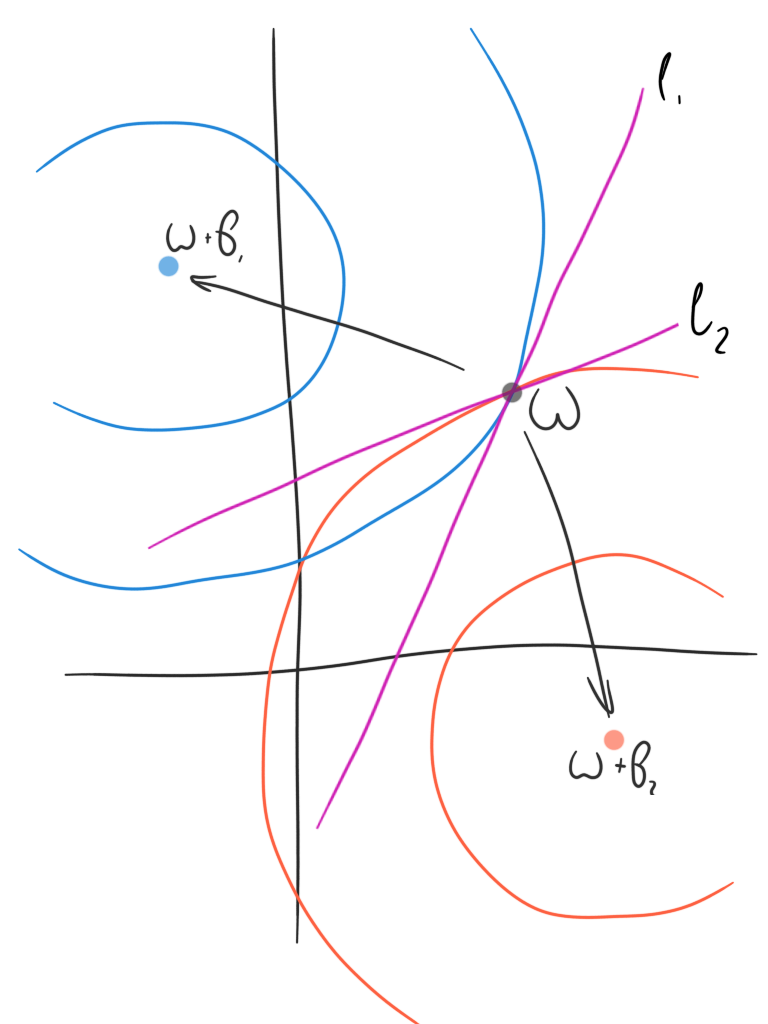
\includegraphics[scale=0.25]{pics/M4/battaglini03.png}
		\caption{Figure 1}
		\label{fig:1}
	}
	\qquad
	\parbox{7cm}{
		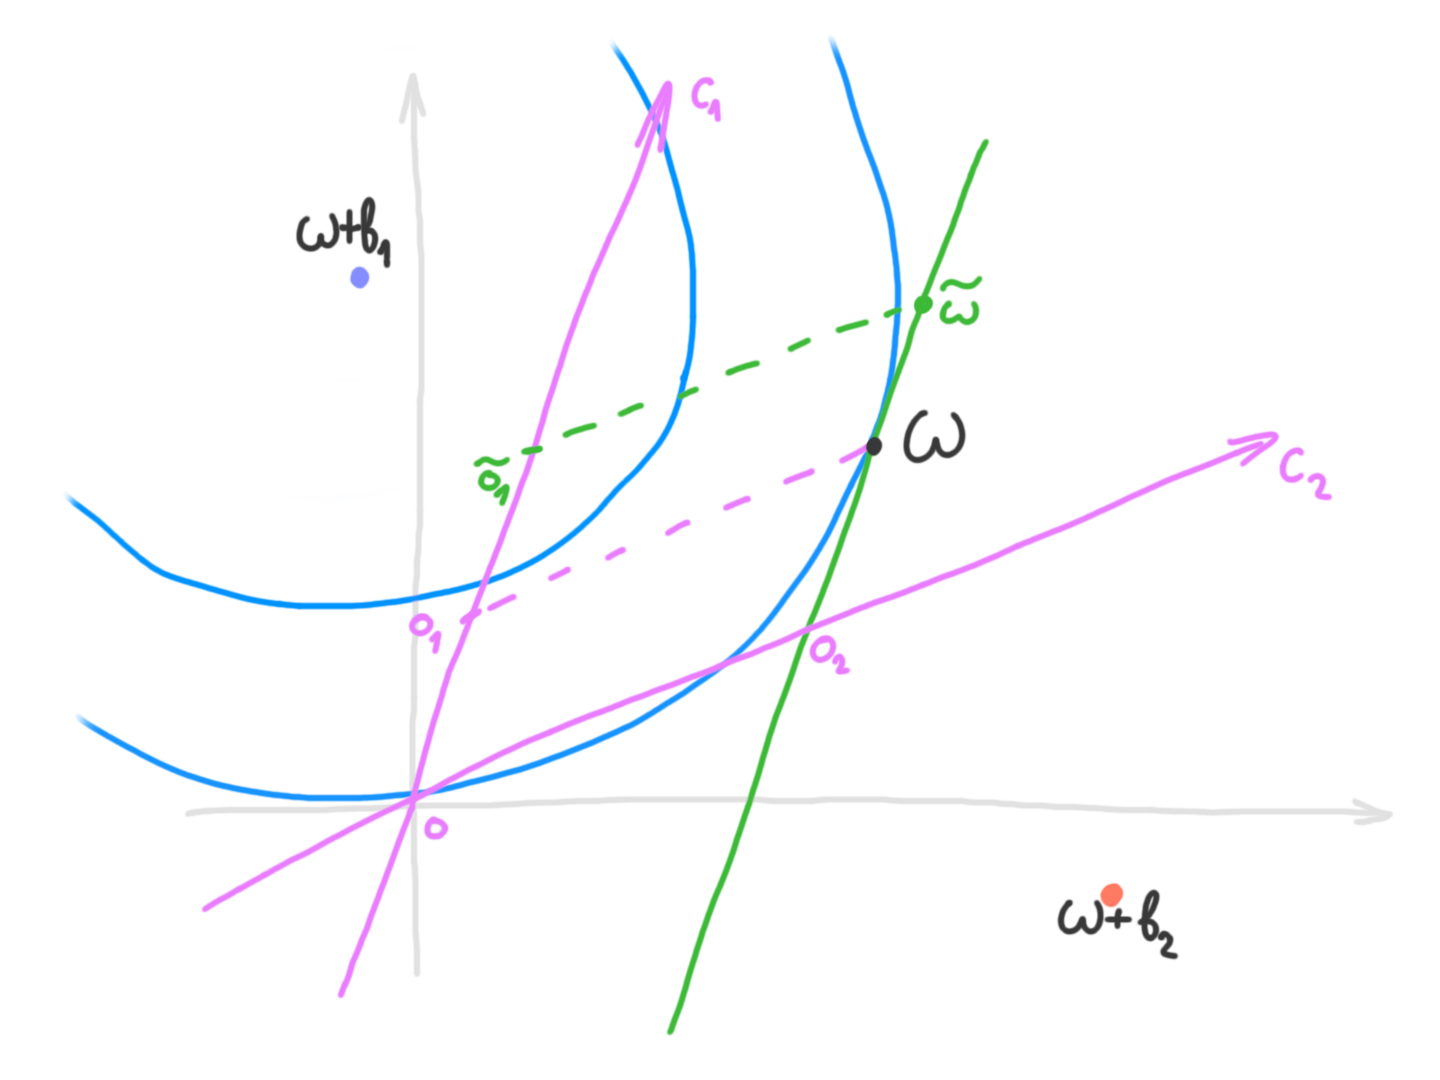
\includegraphics[scale=0.25]{pics/M4/battaglini04.png}
		\caption{Figure 2}
		\label{fig:2}
	}
\end{figure}

Look at Figure \ref{fig:1}. What is the set of actions that should be available to player 1 conditional on player 2 reporting truthfully? In other words, what actions $a$ can player 1 induce through various reports $\hat{m}_1$, given that player 2 follows the prescribed strategy $m_2(\omega)$ (we do not know how it looks yet). For agent 1 to be willing to report truthfully, leading to action $a=\omega$, he must weakly prefer that over all other actions $a$ he can induce -- meaning that the set of such actions must lie outside of the outer blue circle in Figure \ref{fig:1}. In particular, it would be fine if the set of such actions was given by the purple line $l_1$, which is orthogonal to $b_1$. Similarly, the set of actions available to player 2 in equilibrium conditional on P1 following $m_1(\omega)$ can be given by $l_2$, among others.

The question is how we determine the \emph{locations} of these respective lines/action sets. One might think of a kind of two-stage communication mechanism: in stage 1, P1 reports where $l_2$ should be and vice versa, and in stage 2, both players $i$ report where the state is on their respective lines $l_i$. Note, however, that the second stage is redundant: once we know where $l_1$ and $l_2$ are, we already know the state $\omega$ (hint: it is the unique point at which the two lines intersect). But will it actually be an equilibrium for player $i$ to correctly report the location of $l_j$? In fact, yes, since by misreporting player $i$ will only be able to induce actions on $l_i$, which contains no better options for $i$ than the truth. Let us now construct the equilibrium formally.

Consider a basis $(c_1,c_2)$, where $c_i$ is a vector orthogonal to $b_i$ for each $i$.\footnote{E.g., letting $c_i = \frac{1}{\left\| b_i \right\|_2 } \left[ \begin{tabular}{c c} 0 & 1 \\ -1 & 0 \end{tabular} \right] \cdot b_i$ would yield a vector $c_i$ of unit length that is rotated $90\deg$ clockwise w.r.t. $b_i$.}
So long as $b_1$ and $b_2$ are linearly independent, this basis generates the whole linear plane. This means, in particular, that any state $\omega = (\omega^1, \omega^2) \in \mathbb{R}^2$ can be uniquely represented in this basis in terms of pair of coordinates $(o^1, o^2)$, i.e.,
\begin{align*}
	\omega = o^1 \cdot c_1 + o^2 \cdot c_2
\end{align*}
(where $\omega,b_1,b_2$ are all vectors).

Now consider a mechanism in which each player $i$ reports $o^i$.\footnote{Formally, the problem setup says that messages are two-dimensional: $m_i \in \mathbb{R}^2$. So to be 100\% formal you can say that, e.g., $m_i = (o^i, 0)$, and that the principal ignores the second coordinate of each message.}
The principal then takes action $a(o^1,o^2) = o^1 \cdot c_1 + o^2 \cdot c_2$. This decision rule trivially satisfies the principal's optimality condition \eqref{eq:optact} if agents report $o^1$ and $o^2$ truthfully, so we are only left to verify that truth-telling is indeed optimal.

This is best illustrated graphically. Look at Figure \ref{fig:2}. Suppose that P1 reported some $\tilde{o}^1 > o^1$. This would shift the induced action upwards along $l_1$ to $\tilde{\omega}$. We have chosen $l_1$ in such a way that any action on it is worse for P1 than that induced by the truth, hence this deviation is not beneficial for P1. Similar logic applies to any other deviation at the communication stage.


%%-----------------------------------------------------------------------------------------------------

\end{document}
